\documentclass[a4paper,11pt]{scrartcl}
\usepackage{graphicx}
\usepackage{bookmark}
\graphicspath{ {Images/} } 
\usepackage[utf8]{inputenc} 
\usepackage[section]{placeins}
\usepackage{placeins}
\usepackage{amsmath,amssymb,amsthm} 
\usepackage[round]{natbib}
\usepackage{url}
\usepackage{xspace}
\usepackage[left=20mm,top=20mm]{geometry}
\usepackage{algorithmic}
\usepackage{subcaption}
\usepackage{mathpazo}
\usepackage{booktabs}
\usepackage{hyperref}

\title{Math 307 Project - The Traveling Salesman Problem.}
\author{Tino Pimentel, Erik Helm, Austin Hollis}
\date{\today}


\begin{document}

\maketitle

%%%
%

\section{Introduction}

Project:  The TSP problem is defined as follows: Given a set of cities and the distances between each and every pair of cities, find the minimum path that is available to visit all the cities exactly once and then return back to the original starting point. You can imagine the cities as nodes in a connected graph and the straight-line distances as edges between the cities. This is a well known NP-Complete (nondeterministic polynomial time) problem and there are many different heuristics available to obtain approximate solutions.

\section{Abstract}

The Traveling Salesperson (project) problem is when a person wants to travel to every city on the agenda and then return to the original starting city without revisiting any previously traversed city. The next destination chosen to travel to on the grid is logically calculated by finding the minimum distance from the current person’s location to all cities on the agenda. Once the city with the shortest path is determined, the salesperson travels to the city that has the minimal distance to travel while not revisiting previously traveled locations. When the salesperson traverses to the last city, they will then travel back to the starting city from their agenda as a direct path would be the shortest path instead of traveling through previous cities. The process simplified is calculating the Hamilton Circuit from the agenda by adding paths between cities. 
 
\section{BackGround}

The Traveling Salesperson Problem (TSP) is speculated to have originated in 1832 for a tour between Germany and Switzerland. TSP was later formulated by mathematicians W.R. Hamilton and Thomas Kirkman in the 1800s.TSP elevated around 1930 as one of the most thoroughly studied problems in optimization. TSP is still used for benchmarking many optimization methods being developed today. Even though the problem is computationally expensive, a large number of algorithms are known to where  instances with thousands of cities can be solved completely. The algorithms in the most extreme cases can approximate within the one percentile of the exact minimal spanning tree.  

\section{Discussion} 

In the context of graph theory, the general format of the graph will be an undirected weighted graph where incident edges do not have any specific direction for traversing between cities. A weighted graph is a graph in which each edge is assigned a weight.

\begin{itemize}
  \item The vertices(cities) can be modeled as nodes of input size n.
  \item The distance, time, or price traversing between cities can be represented as the weight w for the incident edges between nodes.
  \item A Complete graph $K_n$ is a graph of which all nodes are connected to one another with every node having a degree of n-1 edges due to node not being connected to itself.
  \item Hamilton Circuit for the TSP is a circuit that uses every node of a graph once to form a circuit.
  \item TSP is therefore finding the minimum weight of Hamilton Circuit$K_n$ where every city is connected.
\end{itemize}

The algorithm being explored for assembling the Hamilton Circuit for graph $K_n$ will be the Greedy Algorithm. The Greedy Algorithm is quick and easy, being efficient, however is nonoptimal, due to only comparing neighboring cities under a set maxima and not all other cities, which does not always find the lowest-weight Hamilton Circuit. 
Every designed algorithm is scaled in efficiency by their time complexity in computation. The Time complexity is O($N^2$) (pronounced Big -Oh of N squared) for set amount of cities n to travel to using the Greedy Algorithm due to comparing the current city location to every other neighboring city, every iteration in the algorithm.

\section{Demonstration}

Here an example is demonstrated of the logic for acquiring the Hamilton Circuit for the salesman’s agenda by weight w represented by distance between cities.

\begin{figure}[h!]
  \centering
  \begin{minipage}[b]{0.4\textwidth}
    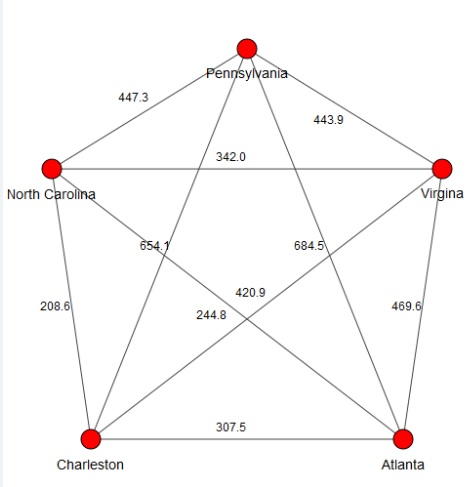
\includegraphics[width=\textwidth]{Step0}
    \caption{Step 0}
  \end{minipage}
  \hfill
  \begin{minipage}[b]{0.4\textwidth}
    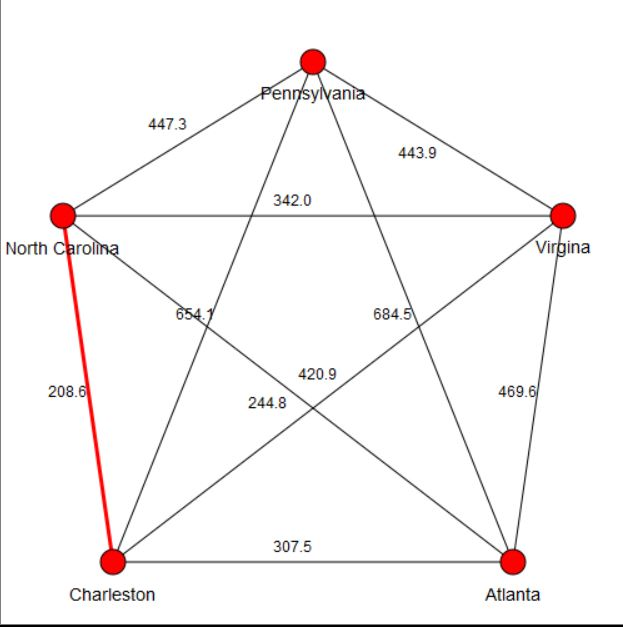
\includegraphics[width=\textwidth]{Step1}
    \caption{Step 1}
  \end{minipage}
\end{figure}

In this example, here we have a salesperson with an agenda to travel to every city in their itinerary starting from Charleston. The salesperson wants to traverse through the list of locations and end back at Charleston without revisiting any other city n. We start by comparing all the distances from Charleston to all other cities under a thousand miles. Once the shortest distance to be traveled from the current city location is located, then the salesperson takes a flight to that city. The salesperson can not travel back to Charleston now, even if Charleston is the shortest path to travel to due to the hamilton circuit concept of graph theory. Therefore, the salesperson only has options of traveling to n-1 cities every step of the way. For example, if the person has four options to choose from and takes a flight, the next time he chooses the next location they will only be choosing from three options. Here every step is highlighted along the way to illustrate the minimum paths taken.

\begin{figure}[h!]
  \centering
  \begin{minipage}[b]{0.4\textwidth}
    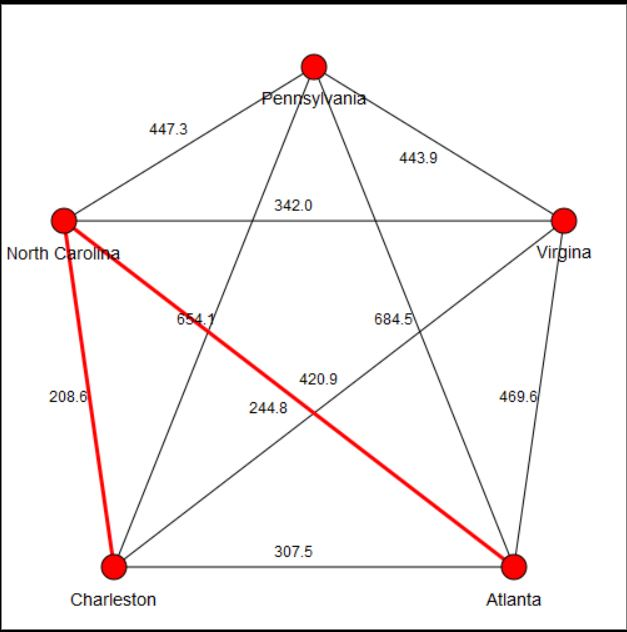
\includegraphics[width=\textwidth]{Step2}
    \caption{Step 2}
  \end{minipage}
  \hfill
  \begin{minipage}[b]{0.4\textwidth}
    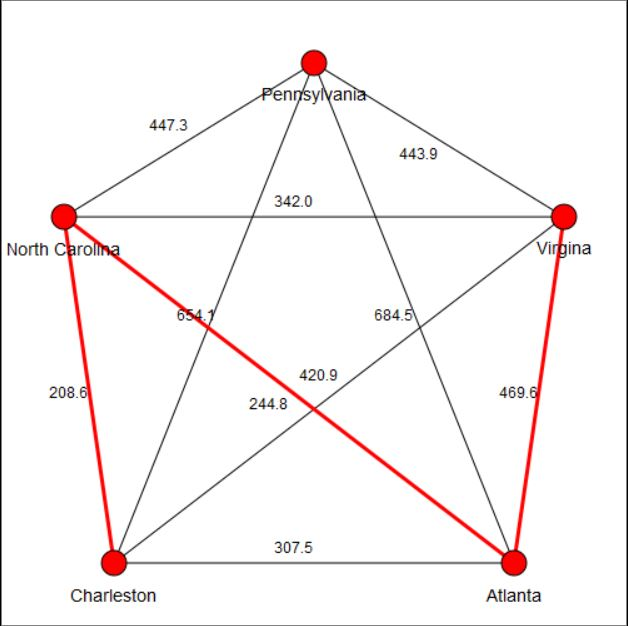
\includegraphics[width=\textwidth]{Step3}
    \caption{Step 3}
  \end{minipage}
\end{figure}

Step 2 and Step 3 illustrates the next iteration through finding the minimum path. Normally the minimum path in Step 3 would to traverse from Atlanta to Charleston, however the definition of a Hamilton circuit in regards to TSP restricts the salesperson to go back to Charleston until all other cities have been visited. Therefore the next minimum path from Atlanta would be Virginia. The salesperson then takes a flight to Virginia, preparing to find the next minimal path from Virginia illustrated in Step 4. Step 4  displays the salesperson not having any other choice for minimal traversal due to the rules for Hamilton circuit in regards to TSP, only being able to succeed to Pennsylvania.

\begin{figure}[!h]
  \centering
  \begin{minipage}[b]{0.4\textwidth}
    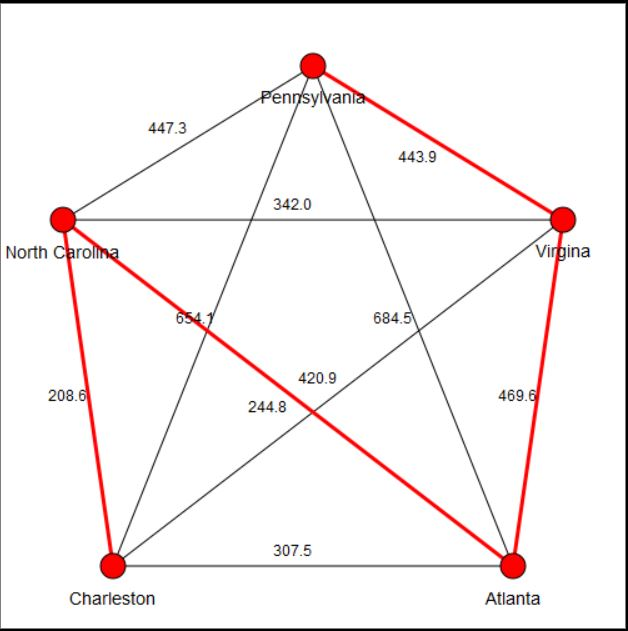
\includegraphics[width=\textwidth]{Step4}
    \caption{Step 4}
  \end{minipage}
  \hfill
  \begin{minipage}[b]{0.4\textwidth}
    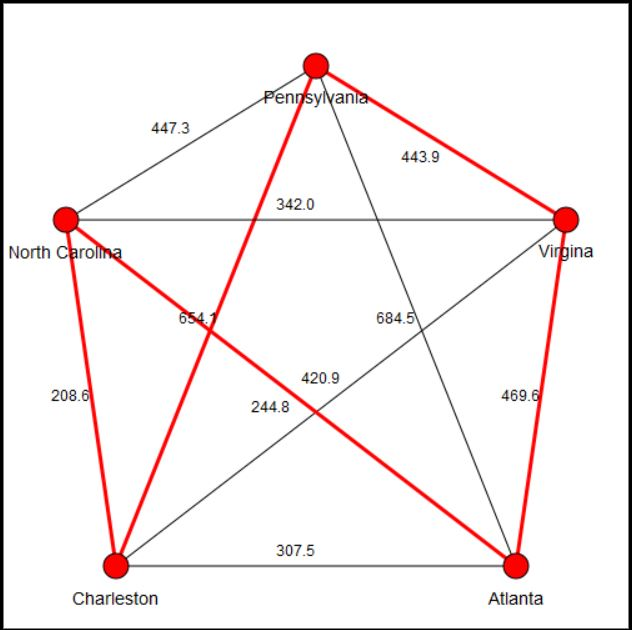
\includegraphics[width=\textwidth]{Step5}
    \caption{Step 3}
  \end{minipage}
\end{figure}

Once the salesperson travels to every city once that is not Charleston, which in this example is illustrated in Step 5, they will then have to travel back to Charleston to finish their journey of travelling around to their locations that are on their agenda.

\section{Computational Analysis}

\begin{figure}[!h]
  \centering
  \begin{minipage}[b]{0.85\textwidth}
    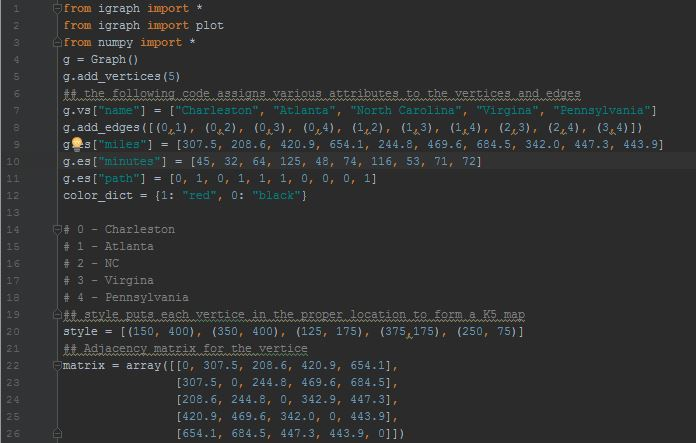
\includegraphics[width=\textwidth]{codepart1}
    \caption{Code Snippet 1}
  \end{minipage}
\end{figure}

\section{Snippet 1}

The programming language used to program the logic of the greedy algorithm is Python. The Python library used to illustrate the previous demonstration is Python-igraph. The data structures involved in the computation for the logic with Python was the Python library NumPy. The libraries for Python have to imported first in order to be utilized throughout the program, as well as their respective methods. In igraph, a graph to start plotting points with vertices is defined as \( $$ g = Graph() $$ \) . Vertices are added with \( $$g.add\_vertices(n)$$ \) for n is the number of cities on the salesman’s agenda as seen in Snippet 1. In Python, counting begins at 0. \( $$g.add\_edges([n_0, n_1, n_2, n_3, n_4])$$ \) \( $$G.vs[]$$ \) refers to the nodes of the created graph, while \( $$g.es[]$$ \) refers to the edges drawn in the graph. The references in igraph to Graph g contain “Attributes” which are just used as visual labels for when Graph g is plotted. style is graph's way of defining the location on the graph where every node (city) will be drawn at. 

\begin{figure}[!h]
  \centering
  \begin{minipage}[b]{0.85\textwidth}
    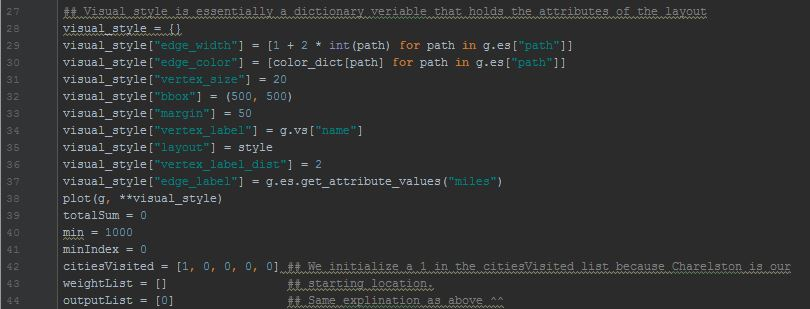
\includegraphics[width=\textwidth]{codepart2}
    \caption{Code Snippet 2}
  \end{minipage}
\end{figure}

\section{Snippet 2}

\(visual\_style[]\) is declared as an empty set from igraph’s layout attributes of the layout of Graph g. \( visual\_style\) also contains attributes within igraph that are being set as an extension of g essentially in Snippet 2.

\begin{figure}[!h]
  \centering
  \begin{minipage}[b]{0.85\textwidth}
    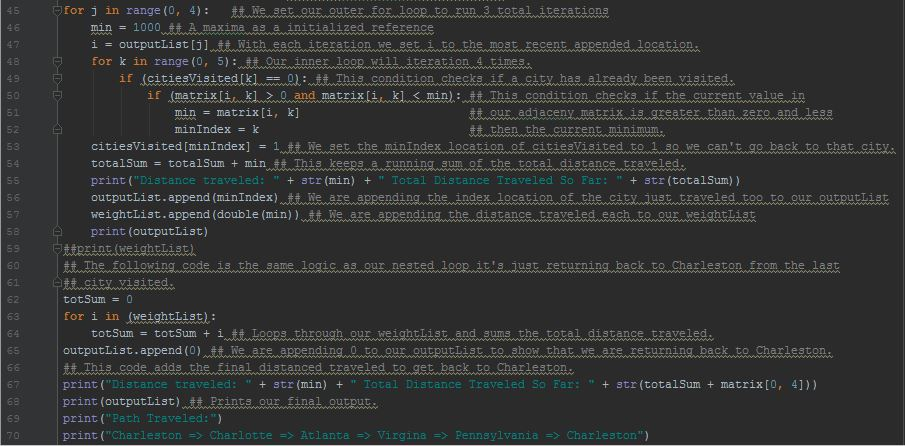
\includegraphics[width=\textwidth]{codepart3}
    \caption{Code Snippet 3}
  \end{minipage}
\end{figure}

\section{Snippet 3}

The maxima variable in Snippet 2 labeled min set as 1000 is essential with the nested for loop in Snippet 3. The NumPy method for adjacent matrices is filled with the distances in reference to every node in Graph g (Snippet 2). The nested for loop calculates the most minimal path by comparing the distances between all edges from the location the salesperson is currently at within the j counter of the first for loop, to the rest of the locations in Graph g through the 2nd for loop k counter. The adjacent matrix is referenced to with index value of j and k as the new min. While the nested for loop runs through calculating the shortest paths throughout Graph g, the total distance traveled is accumulated with totalSum.  After every j iteration in the for loop, the minimal index value is added to outputList, in order to keep track of the order the salesperson traversed through the cities.  The min value, when referenced from the matrix of distances, is the distance of the shortest path between two cities and is added to its own weightList in order to keep track of the weights that will be added to totalSum. Every comparison for the minimum path between two cities is also checked back with the citiesVisited list to prevent an already visited city to not be added to the outputList. The print statements near the bottom of Snippet 3 are for illustrating every step of the way for traversing through the Hamilton Circuit of Graph g after the nested for loop from the accumulating lists outputList.


\begin{figure}[!h]
  \centering
  \begin{minipage}[b]{0.85\textwidth}
    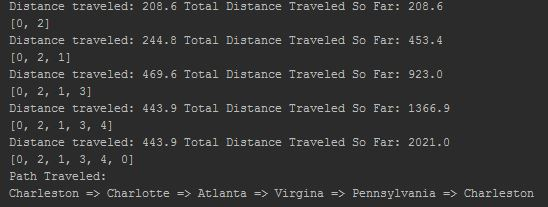
\includegraphics[width=\textwidth]{igraphprojectsnippet}
    \caption{Code Snippet Results}
  \end{minipage}
\end{figure}

\section{Computational Results}

The first distance traveled represents the distance traveled from the city at the current iteration to the next city determined as the minimum path. The second distance traveled so far result is the accumulated distance traveled throughout the journey. Every iteration the salesperson travels, the journey is displayed progressively by the numerical representations of the nodes. The journey is then converted from its numerical representation to their respective city names.

\section{Conclusion}

In conclusion, an algorithm for TSP can be computed with finding a Hamilton circuit with an input of n cities, which include set weight w for potentially either distance, price, or time between cities. The Greedy Heuristic (approximation) Algorithm seems feasible, by calculating a reasonable minimal path between cities once a minimum between two cities has been devised with set maxima. Modern methods can find solutions for extremely large problems (millions of cities) within a reasonable time which are with a moderate probability within a 25\% approximation of the optimal solution being obtained from the Greedy Algorithm. Solutions to TSP possess applications in problems such as optimizing airline routes or laying cables, and even DNA or genome research.

\section{Bibliography}

"World Traveling Salesman Problem." World Traveling Salesman Problem. N.p., n.d. Web. 23 Apr. 2017. <http://www.math.uwaterloo.ca/tsp/world>.\newline
\newline
Johnson, David S., and Lyle A. McGeoch. "Review: The Traveling Salesman Problem: A Guided Tour of Combinatorial Optimization." The Journal of the Operational Research Society 37.5 (1986): 535-36. The Traveling Salesman Problem: A Case Study in Local Optimization. Web. 21 Apr. 2017. <https://www.cs.ubc.ca/~hutter/previous-earg/EmpAlgReadingGroup/TSP-JohMcg97.pd>.\newline
\newline
"Welcome to Python.org." Python.org. N.p., n.d. Web. 20 Apr. 2017. <http://www.python.org/>.\newline
\newline
"Get Started with Python-igraph." Python-igraph. N.p., n.d. Web. 18 Apr. 2017. <http://igraph.org/python/>.\newline
\newline
"NumPy¶." NumPy — NumPy. N.p., n.d. Web. 18 Apr. 2017. <http://www.numpy.org/>.\newline



\end{document}